% TEMPLATE for Usenix papers, specifically to meet requirements of
%  USENIX '05
% originally a template for producing IEEE-format articles using LaTeX.
%   written by Matthew Ward, CS Department, Worcester Polytechnic Institute.
% adapted by David Beazley for his excellent SWIG paper in Proceedings,
%   Tcl 96
% turned into a smartass generic template by De Clarke, with thanks to
%   both the above pioneers
% use at your own risk.  Complaints to /dev/null.
% make it two column with no page numbering, default is 10 point

% Munged by Fred Douglis <douglis@research.att.com> 10/97 to separate
% the .sty file from the LaTeX source template, so that people can
% more easily include the .sty file into an existing document.  Also
% changed to more closely follow the style guidelines as represented
% by the Word sample file. 

% Note that since 2010, USENIX does not require endnotes. If you want
% foot of page notes, don't include the endnotes package in the 
% usepackage command, below.

% This version uses the latex2e styles, not the very ancient 2.09 stuff.
\documentclass[letterpaper,twocolumn,10pt]{article}
\usepackage{usenix,epsfig,endnotes,placeins}
\begin{document}

%don't want date printed
\date{}

%make title bold and 14 pt font (Latex default is non-bold, 16 pt)
\title{\Large \bf SSID's and Social Networks}

%for single author (just remove % characters)
\author{
{\rm Michael Ballantyne}\\
University of Utah
\and
{\rm Maria Jenkins}\\
University of Utah
% copy the following lines to add more authors
\and
{\rm Priyanka Parekh}\\
University of Utah
} 

\maketitle

% Use the following at camera-ready time to suppress page numbers.
% Comment it out when you first submit the paper for review.
\thispagestyle{empty}


\subsection*{Abstract}
Some Wi-Fi network clients transmit a list of networks they've
previously connected to when scanning for networks to join, and many
users are not aware that this data is broadcasted and can be easily
monitored. We hope to make users aware that this data can reveal
information about locations they spend time and their social
connections. We captured Wi-Fi probe requests from a sample of
wireless clients and analyzed the social network implied in the data
for privacy risks. We found that Apple laptops revealed the most,
while most mobile devices and computers running Linux no longer share
private data in probe requests. The data suggests that while some
computers no longer reveal previous network associations, large scale
data from the remaining clients could present a significant privacy
risk. Even at small scale the list of network associations is a
possible tool for Wi-Fi client fingerprinting. Our work concurs with
other recent studies showing that network associations can be used to
fingerprint Wi-Fi clients or link users to certain political organizations or other groups based on the names of the networks. To encourage
users to be more security conscious we provided participants with a
personalized interactive social network graph showing how their
network associations relate them to other participants. We include
results from a survey conducted to understand participants' reactions
to this data.

\section{Introduction}
Laptops broadcast the list of Wi-Fi networks (SSID's) that a user has ever connected to. The list of SSID's is broadcasted when your laptop is attempting to connect to a Wi-Fi hotspot (access point). Wi-Fi access points are ubiquitous and passive Wi-Fi tracking has started to gain popularity amongst retailers, advertisers, and data analytics companies to glean useful information about people. A quick google search for passive Wi-Fi tracking reveals tutorial after tutorial on how to conduct passive Wi-Fi tracking. It is a trivial undertaking to extract this data while it's being broadcasted.  

Previously cell phones broadcasted this data however recently they have stopped. A large majority of users are unaware that this metadata is being publicly broadcast and can be easily collected. The fact that this data is being broadcasted raises privacy and security concerns. Your SSID list is a form of location history. From your SSID list it could be inferred what your favorite coffees shop is, what conferences you attend, your social and political affiliations and where you work among other things. It also raises some security concerns. An attacker who captures this information could conduct a man-in-the-middle attack, an evil twin attack or Auto Association Karma Attack [Reference] to name a few. 

In contrast to recent work in this area this paper focuses on the broadcast of SSID's from laptops attempting to connect to a Wi-Fi access point. We will demonstrate how this data can be collected and used to imply social networks. We will explore the privacy and security implications of this publicly broadcasted metadata. We do so by collecting data from Wi-Fi access points and rendering social network graphs and examining the connections. In section 2 we discuss Wi-Fi network scanning. In section 3 we mention related work in this area. From section 4 onwards we discuss our study methods, results, and conclude.



\section{Background}
Every wireless enabled device has to go through a discovery process to connect to a Wi-Fi access point. Devices can use passive or active discovery to connect to an access point. There are three specific types of scans a device can deploy. The first falls under the active scan category. A client sends a directed probe request with the list of SSID's to the access point in plain text. The second active scan is a broadcast probe. The broadcast probe  sends the MAC address of the clients device and asks for information on all the networks. There is a passive scan where the client waits for beacon frames. Beacon frames are packets that are broadcast by the Wi-Fi access point and the device waits for a frame from an access point it has previously connected to. 

Different laptops use different probe request methods. Cell phones use a mixture of broadcast probes and passive scanning. To gather this data is trivial with access to a computer or Wi-Fi device. The laptop or Wi-Fi device can be put into monitor to pickup nearby traffic. In doing so the device in monitor mode is not broadcasting its presence, making it hard to detect if a nearby user is collecting your metadata.

\section{Related Work}
There is a fairly large body of work investigating the utility of metadata that is broadcast when connecting to Wi-Fi access points. The majority of the work was targeted at cell phones and not laptops. Recently cell phones have stopped broadcasting the SSID list when probing for Wi-Fi connections.

Cheng et al \cite{cheng} sought to discover user relationships from observing the similarity of SSID lists between users, they took into account physical proximity and spatio-temporal behavior. They looked at the similarities of SSID lists being broadcast from cell phones before cell phones disabled this feature. They found that spatio-temporal data had more social connections. They believed their work could be applied to research in social ties and the deployment of wireless networks.

Barbera et al \cite{barbera} used social network analysis on datasets of Wi-Fi probes from cell phones in public areas. They found that data matched typical properties of social networks. They also mentioned what devices broadcast the SSID list when probing for a connection.

Desmond et al \cite{desmond} discussed an alternative approach to fingerprinting that defeats MAC address 
randomization and the absence of an SSID list by timing the intervals between Wi-Fi probes, but requires hours of continuous data to perform adequately. Their results indicated that this technique is accurate in differentiating between unique devices. Their approach is different from other technique because it is passive and non-invasive.

Cunche et al \cite{cunche}  present a mechanism to detect links between people by fingerprinting devices by exploiting the fact the SSID lists are broadcast in plain text when probing for WI-FI connections. They take a very quantitative approach and are able to gather a large data set. This work demonstrates a privacy breach allowed by the 802.11 probe requests and raises awareness that initiative should be taken to increase privacy in terms of access point discovery. 

Greenstein et al \cite{greenstein} makes the argument that it is in the best interest of not only users, but also manufacturers, to address the privacy threats that wireless networks pose. The authors considered an 802.11 case study and analyzed 802.11 traces. They used this information to show that, over time, devices can be identified and tracked through its SSID lists, its persistent link-layer address, and other characteristics. The authors of this work provide suggestions for ways to improve privacy through design considerations.

\section{Privacy Considerations}
To conduct this study we had to take into consideration the security and privacy of our participants so as to minimize harm but still collect meaningful data. The intent of our project is to reveal the potential privacy implications of the type of data we collected, so we had to address the reasonable privacy concerns of our participants.

\subsection{Location Data}
While we didn't directly collect location history, the names of wireless networks often identify a location. The name itself might describe the location, like the name of a business or airport. It might also be recorded in a database of wireless networks. Companies like Apple and Google use such databases to geolocate devices based on surrounding wireless networks but there are also publicly available databases assembled by hobbyists. All sorts of networks including homes, workplaces, and social locations like coffee shops are included in these databases. One such publicly available database is wiggle.net. Figure~\ref{wiggle} shows the location associated with one of the networks that appeared in our study.

\begin{figure*}
\centering
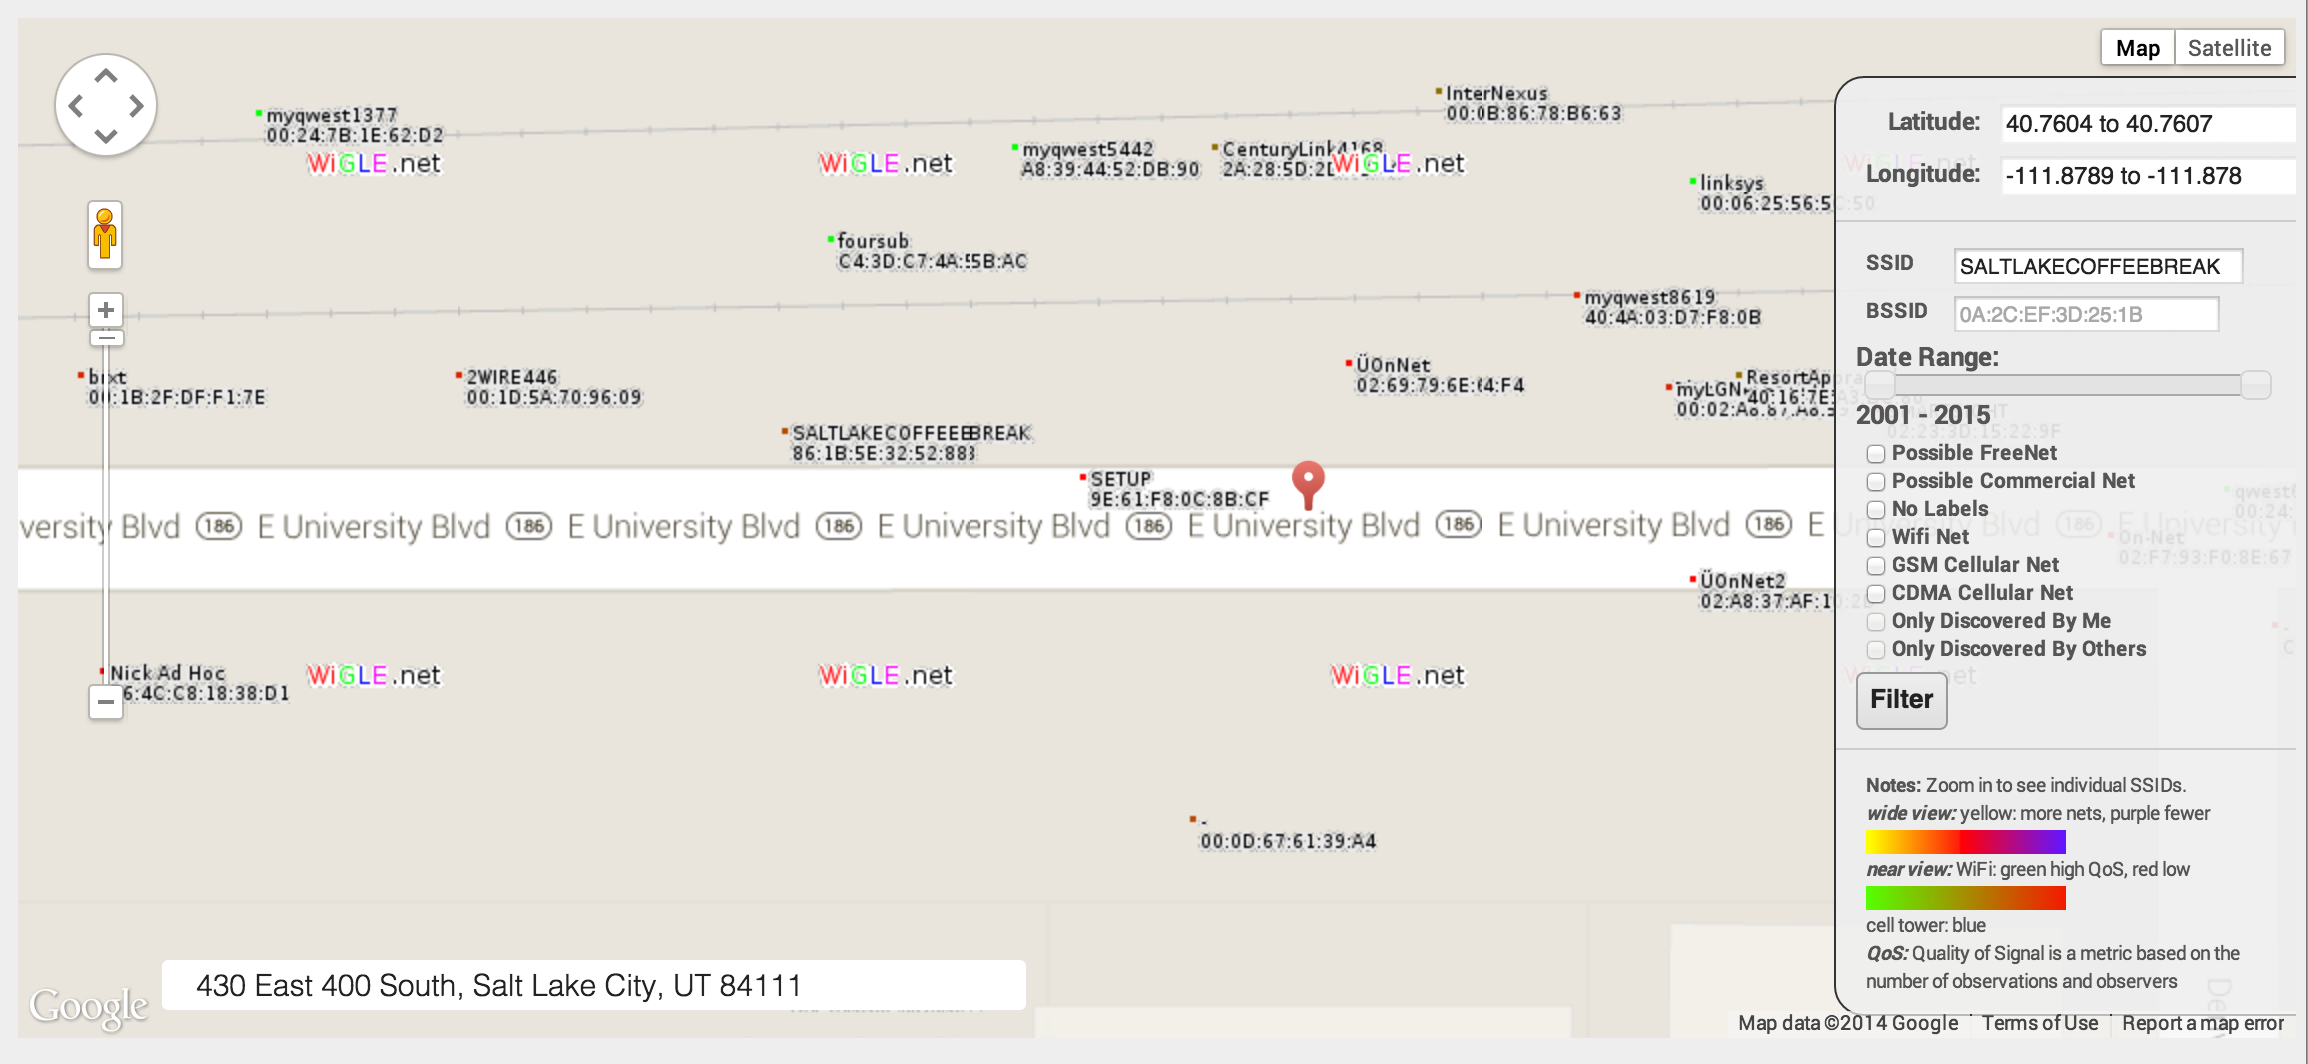
\includegraphics[scale=.43]{wigle}
\caption{\textsf{Coffee Break's Wi-Fi access point location}}
\label{wiggle}
\end{figure*}




\subsection{De-identification}
Other participants have information to de-identify

De-identification risks in time-series data

\subsection{Other Risks}
We took precautionary measures to protect the anonymity of our users and the data we collected from them. All participants in the study were required to opt in to the study by signing an informed consent. The informed consent notified the participants what data we would be collecting, how we would use it, and what our data retention policies were. 

Personalized social network graphs created another privacy risk for our study. We did not want any other participants to be able to identify other nodes on the graph. We decided that only showing the networks that two or more participants had connected to would reduce this risk. We also did not look at the data when generating the graphs.



\section{Data Collection}
Because of the privacy concerns discussed above, we decided to only collect SSID lists from those who actively chose to participate in to the study. We also decided against using time series data.

In the original design of our study, we had planned to collect data from a public location in a university building for up to a week. We needed a device to capture packets that was inexpensive and could be easily concealed to guard against theft. We also wanted to ensure that the device wouldn't hold previously captured data so that nothing about participants could be revealed in the event of theft. Our tool of choice was the Wi-Fi Pineapple, a small dual radio wireless access point designed for penetration testing. The second radio lets the Pineapple connect to a normal Wi-Fi network to communicate with our server to receive commands and return the captured data. We configured the Pineapple to establish an ssh connection and reverse port forward on a server on Amazon Web Services. Then the server controlled the Pineapple on an ssh connection through the reverse tunnel. Captured packets were immediately forwarded through the SSH connection to the server so that no participant data was persistently stored on the Pineapple.

We captured and filtered packets on the Pineapple with the scapy python library to minimize the amount of data that we had to backhaul to the server. As discussed in section~\ref{bpf}, we would have done better to filter packets in the kernel with linux socket filtering to improve performance. On the server we stored the collected SSID lists in sqlcipher, an AES-256 encrypted version of sqlite. All of our access to the collected data was mediated by Python scripts that limited the data that we could see according to the privacy rules we defined in our informed consent document, and the participant reports were similarly assembled and sent programmatically to limit our exposure to private participant data.

\section{Data Evaluation}
We were less successful in capturing data than we anticipated. Of our 28 participants (including the authors), 18 only yielded zero or one network name. Figure~\ref{histogram} shows the full distribution of network counts. Following data collection, we performed some further experiments to explain these disappointing results.

\begin{figure}
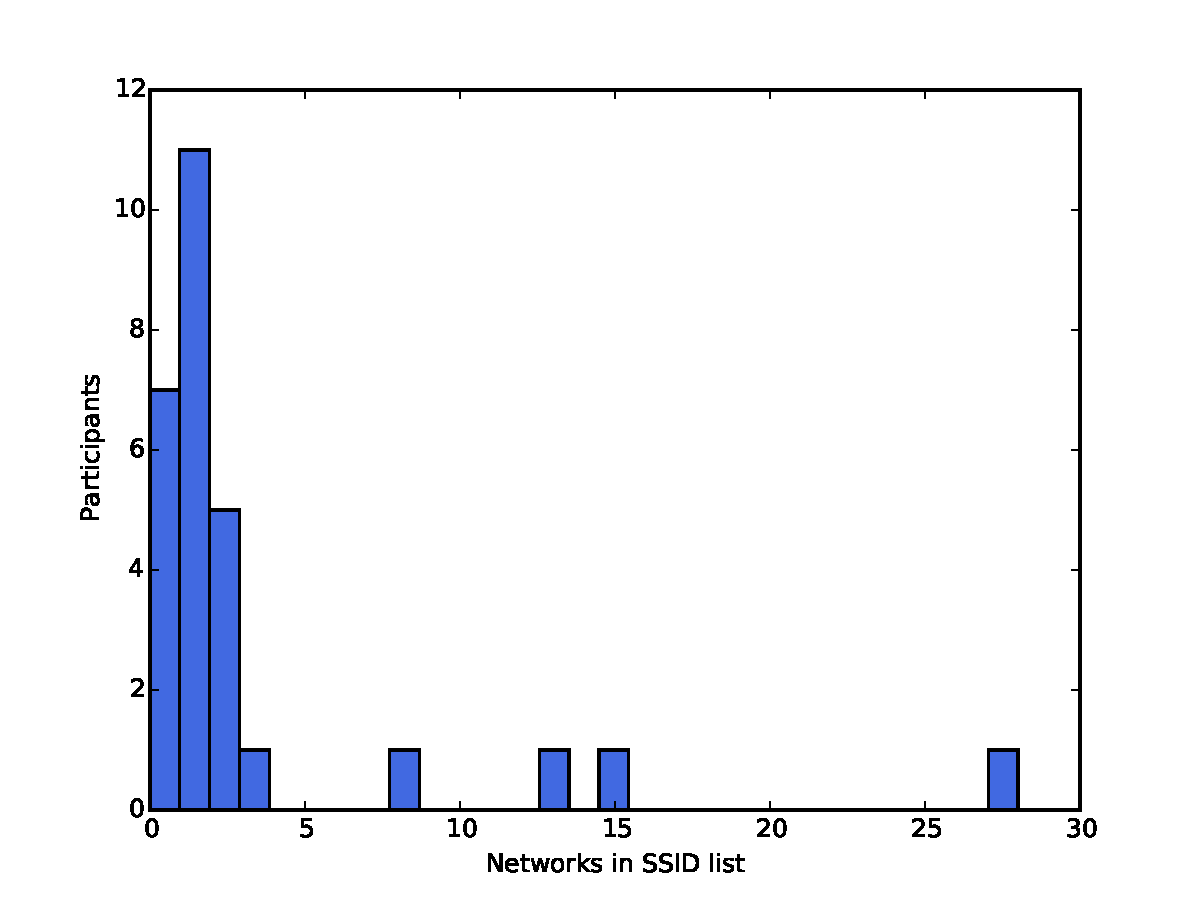
\includegraphics[width=\columnwidth]{hist.pdf}
\caption{Histogram of SSID list size}
\label{histogram}
\end{figure}

\FloatBarrier

\subsection{Capture Reliability}
The three individuals yielding the most network names were the authors. We hypothesize that more complete network lists were collected from our devices because they were present near the monitoring device for an extended period of time, so there were multiple opportunities to capture the data. As a test we measured the number of network names cumulatively collected by packet capture while a MacBook scanned for wireless networks a number of times. We found that a capture of only a single scan yielded on average only 31\% of the network list (with 28 networks total) and that we'd need to capture four or five scans to get a mostly-complete list. Figure~\ref{scans} shows the complete results of this experiment. An attacker able to monitor traffic over a long period of time likely wouldn't find this to be a problem, but it might thwart reliable fingerprinting of clients an access point only sees once. However, we suspect that our failure to capture the SSID list reliably was not because they were not transmitted, but because our receiver was overwhelmed and unable to keep up with filtering.

\subsection{Linux Socket Filtering}
\label{bpf}
During packet capture with scapy we found that the Wi-Fi Pineapple occasionally froze, requiring a restart, and at other times took several seconds to register new packets. We suspect that our packet filtering code in python wasn't able to keep up with the volume of captured packets. The Pineapple only has a 400 MHz processor, and each packet received must be communicated from kernel-space to user-space by a system call before it is filtered in python. Sometime after the data collection phase of our project we learned about linux socket filtering, a way to filter packets in kernel-space before they are returned to a packet monitoring application. Filters from tools like tcpdump typically use this method. The filtering rules available through tcpdump are sufficient to express the filter we'd written in scapy. Testing with tcpdump filtering shows that it reliably collects at least 16 of 28 networks from a single scan. It isn't clear why only 16 of the network names appear to be transmitted during a scan. Perhaps the laptop successfully established a connection before needing to complete the scan; more seem to be transmitted when initially enabling wireless in a location where none of the remembered wireless networks are available. Overall we suspect that if we'd used kernel level filtering during the data collection phase of our study we would have collected more network names from some of our participants.

\subsection{Operating System Behavior}
Another factor limiting the volume of data we captured was encouraging --- it appears that Linux and Windows clients don't generally perform directed probes, opting instead for broadcast probes unless a network was specially configured. During data collection we noted that captures from devices running Linux usually only included a single SSID plus a broadcast probe. The final social network graph discussed in section~\ref{social} shows many devices only having connected to UConnect, the campus wireless network. We hypothesize that Linux devices transmit directed probes only for the network they're currently connected to or were most recently connected to. Other networks are discovered by broadcast probes. Documentation for wpa\_supplicant on linux suggests that users could configure individual networks for which directed probes should be used, like hidden networks, but that otherwise it would use broadcast probes. We haven't found documentation for the behavior on Windows but we suspect that it similarly only uses directed probes for manually configured networks that may be hidden. Of the 5 devices in our study that yielded 3 or more network names, all were Apple devices. At least one of those devices was running the latest release of OS X, Yosemite.

These results suggest that vendors other than Apple have recognized the security and privacy implications of directed probes and modified their devices to instead use broadcast probes. Our testing suggests that Apple has done the same for its mobile devices, but not for OS X. Given that other platforms have demonstrated that broadcast probing works effectively we argue that Apple should change the behavior of OS X to better preserve privacy.
\begin{figure*}
\centering
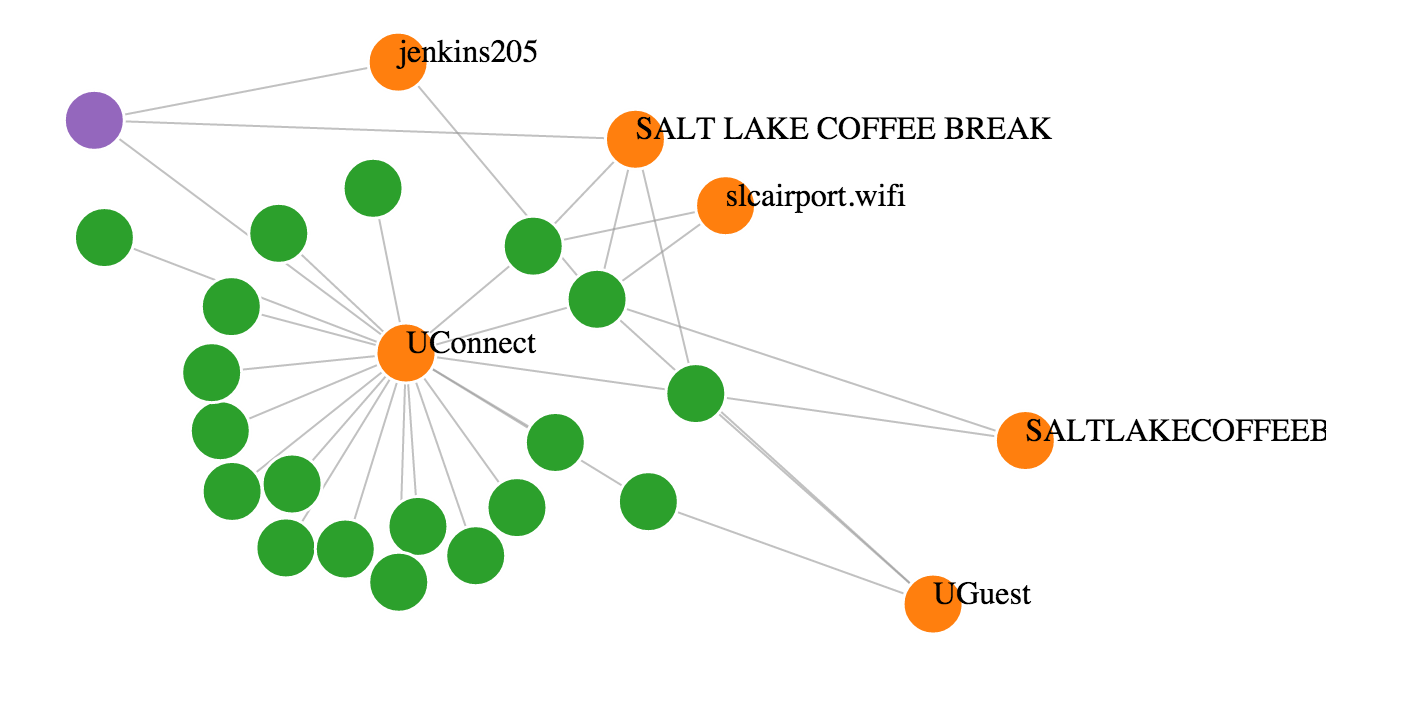
\includegraphics[scale=.5]{graph.png}
\caption{\textsf{Social network graph}}
\end{figure*}
\begin{figure}
\centering
\begin{tabular}{l | l}
Scans & SSIDs Collected \\ 
\hline
1 & 31\% \\
2 & 53\% \\
3 & 63\% \\
4 & 89\% \\
5 & 91\% \\
\end{tabular}
\caption{SSID collection by number of network scans captured. Full SSID list is 29 networks. Averaged over 3 trials.}
\end{figure}


\section{Social Network Analysis}

SSID lists and MAC addresses can be used to infer social networks and ties\cite{cheng}. Although we didn't gather enough data to infer large social networks we gathered enough to construct a graph of the participants and the SSID's the participants had in common. The filtered metadata was used to create personalized social network graphs for each participant. The graphs were rendered using Javascripts D3 library. The graphs were rendered and sent out to participants with an automated script so that their complete SSID lists and graphs were never looked at. 

Figure 2 is an example social network graph. The green nodes denote the anonmyized participants, the purple node indicates the participant, and the orange nodes denote the SSID's shared among participants. Along with the graph the list of SSID's that was broadcast by the participants laptop was included. They are not pictured here to protect this individuals privacy. Wi-Fi access points were only included if more than two users had connected to them. We promised not to include the home network names and only one home network name had at least two participants that had connected to it. The network happened to be one of the authors home networks so we received authorization to include it in the network graph. 

The nodes on our graph are what we anticipated. A mixture of University access points, coffee shops, and airports. From this graph we could infer that some students of the University of Utah frequent Coffee Break and have traveled outside of Salt Lake by airplane. While the information we gathered is rather benign, larger data collection and social network analysis is viable and could reveal much more meaningful information. 

\section{Implications}


\subsection{Location Narrative}
Wigle.net

Locational narrative 

\subsection{Client Fingerprinting}

We wanted to look at fingerprinting participants based upon their SSID lists. We thought that based upon the different networks participants have connected to the lists would be different enough that we could uniquely identify participants. While the lists in our study were unique from one another we did not gather near enough data to conclusively say it is possible to fingerprint solely based upon your SSID list. We leave this for future work.

Related works in this area have successfully fingerprinted devices and inferred social networks from the similarities of these fingerprints. One such work noted that it was possible to infer relationships from the SSID list similarities and grouped participants with similar SSID lists into groups to infer social ties\cite{cunche}. Two other works successfully fingerprinted using the timing of the probe request frames \cite{desmond} and the waveform \cite{ureten}. These works focus more on security than privacy.


\section{Participant Survey}


To gauge our participants reactions we asked our participants to complete a survey after viewing their personalized social network graph. The survey included three questions. The first being did you know prior to our project that your SSID list is broadcast when you probe to connect to a Wi-Fi network? The second was what are you reactions to your personalized study results? The third question was not mandatory. It was what are you reactions to this study in general? We did not receive responses from the majority of our participants. Every participant that did respond said they did not know this data was broadcast. The last two questions were to gauge the sentiment of our participants. The answers gave us the sense that it didn't matter to them that their data was broadcast but they could see the utility of the metadata for advertisers.


\section{Future Work}
While it appears that directed probing is on the decline, Wi-Fi networks still present other security and privacy concerns. Future work is needed to measure these risks and develop improved wireless protocols that are more secure and provide improved guarantees of privacy. As vendors move away from directed probing they usually move to broadcast probes. Broadcast probes don't reveal a list of remembered networks, but they do reveal the MAC address of the client. MAC addresses from probes are increasingly used to track people through physical spaces. IOS 8 is reported use a randomized MAC address for probes, but we aren't aware of a study examining the prevalence of MAC address randomization in non-Apple devices. Even given MAC randomization in probes, devices generally reveal their true MAC address when associated with a wireless network. It should be possible to design a wireless protocol in which no unique identifier is transmitted in the clear. Devices would only share a unique identifier after establishing an encrypted connection with an access point. Such a protocol could limit device fingerprinting to much less accessible physical layer attacks measuring the characteristics of wireless radios.

\section{Conclusion}



\bibliographystyle{acm}
\bibliography{references}


\end{document}